\documentclass[12pt,onecolumn]{article}
\usepackage[utf8]{inputenc} % UTF8 input encoding
\usepackage[T2A]{fontenc}   % T2A font encoding for Cyrillic script
\usepackage[russian]{babel} % Russian language support
\usepackage{listings}
\usepackage{float}
\usepackage{mathtools}
\usepackage{longtable}
\everymath{\displaystyle}
\usepackage{listings} 
\usepackage[usenames]{color}
\usepackage[html]{xcolor}
\usepackage{framed}
\usepackage{csquotes}
\usepackage{geometry}
\usepackage{fancyvrb}
\usepackage{sverb}

\geometry{
  a4paper,
  top=20mm, 
  right=20mm, 
  bottom=20mm, 
  left=25mm
}

\definecolor{mygreen}{rgb}{0,0.6,0}
\definecolor{mygray}{rgb}{0.5,0.5,0.5}
\definecolor{mymauve}{rgb}{0.58,0,0.82}
\definecolor{terminalbgcolor}{HTML}{330033}
\definecolor{terminalrulecolor}{HTML}{000099}
\newcommand{\lstconsolestyle}{
\lstset{
	basicstyle=\color{black}\linespread{1.15}\fontfamily{fvm}\scriptsize\selectfont,
	breakatwhitespace=false,  
	breaklines=true,
	captionpos=b,
	commentstyle=\color{mygreen},
	deletekeywords={...},
	escapeinside={\%*}{*)},
	extendedchars=true,
	frame=single,
	keepspaces=true,
	keywordstyle=\color{blue},
	%language=none,
	morekeywords={*,...},
	numbers=left,
	numbersep=5pt,
  framerule=1pt,
	numberstyle=\color{mygray}\tiny\selectfont,
	rulecolor=\color{terminalbgcolor},
	showspaces=false,
	showstringspaces=false,
	showtabs=false,
	stepnumber=2,
	stringstyle=\color{mymauve},
	tabsize=2,
  literate={а}{{\selectfont\char224}}1
  {б}{{\selectfont\char225}}1
  {в}{{\selectfont\char226}}1
  {г}{{\selectfont\char227}}1
  {д}{{\selectfont\char228}}1
  {е}{{\selectfont\char229}}1
  {ё}{{\"e}}1
  {ж}{{\selectfont\char230}}1
  {з}{{\selectfont\char231}}1
  {и}{{\selectfont\char232}}1
  {й}{{\selectfont\char233}}1
  {к}{{\selectfont\char234}}1
  {л}{{\selectfont\char235}}1
  {м}{{\selectfont\char236}}1
  {н}{{\selectfont\char237}}1
  {о}{{\selectfont\char238}}1
  {п}{{\selectfont\char239}}1
  {р}{{\selectfont\char240}}1
  {с}{{\selectfont\char241}}1
  {т}{{\selectfont\char242}}1
  {у}{{\selectfont\char243}}1
  {ф}{{\selectfont\char244}}1
  {х}{{\selectfont\char245}}1
  {ц}{{\selectfont\char246}}1
  {ч}{{\selectfont\char247}}1
  {ш}{{\selectfont\char248}}1
  {щ}{{\selectfont\char249}}1
  {ъ}{{\selectfont\char250}}1
  {ы}{{\selectfont\char251}}1
  {ь}{{\selectfont\char252}}1
  {э}{{\selectfont\char253}}1
  {ю}{{\selectfont\char254}}1
  {я}{{\selectfont\char255}}1
  {А}{{\selectfont\char192}}1
  {Б}{{\selectfont\char193}}1
  {В}{{\selectfont\char194}}1
  {Г}{{\selectfont\char195}}1
  {Д}{{\selectfont\char196}}1
  {Е}{{\selectfont\char197}}1
  {Ё}{{\"E}}1
  {Ж}{{\selectfont\char198}}1
  {З}{{\selectfont\char199}}1
  {И}{{\selectfont\char200}}1
  {Й}{{\selectfont\char201}}1
  {К}{{\selectfont\char202}}1
  {Л}{{\selectfont\char203}}1
  {М}{{\selectfont\char204}}1
  {Н}{{\selectfont\char205}}1
  {О}{{\selectfont\char206}}1
  {П}{{\selectfont\char207}}1
  {Р}{{\selectfont\char208}}1
  {С}{{\selectfont\char209}}1
  {Т}{{\selectfont\char210}}1
  {У}{{\selectfont\char211}}1
  {Ф}{{\selectfont\char212}}1
  {Х}{{\selectfont\char213}}1
  {Ц}{{\selectfont\char214}}1
  {Ч}{{\selectfont\char215}}1
  {Ш}{{\selectfont\char216}}1
  {Щ}{{\selectfont\char217}}1
  {Ъ}{{\selectfont\char218}}1
  {Ы}{{\selectfont\char219}}1
  {Ь}{{\selectfont\char220}}1
  {Э}{{\selectfont\char221}}1
  {Ю}{{\selectfont\char222}}1
  {Я}{{\selectfont\char223}}1
}
}

\lstdefinestyle{c}{language=C, 
  basicstyle=\small\ttfamily,
  commentstyle=\color{cyan},
  stringstyle=\color{magenta}\ttfamily,
  keywordstyle=\color{blue},
  numbers=left,
  numberstyle=\scriptsize,
  numbersep=5pt,
  frame=single,
  breaklines=true,
  breakatwhitespace=true,
  showstringspaces=false,
  tabsize=4,
  inputencoding=utf8,
  extendedchars=true,
  literate={а}{{\selectfont\char224}}1
          {б}{{\selectfont\char225}}1
          {в}{{\selectfont\char226}}1
          {г}{{\selectfont\char227}}1
          {д}{{\selectfont\char228}}1
          {е}{{\selectfont\char229}}1
          {ё}{{\"e}}1
          {ж}{{\selectfont\char230}}1
          {з}{{\selectfont\char231}}1
          {и}{{\selectfont\char232}}1
          {й}{{\selectfont\char233}}1
          {к}{{\selectfont\char234}}1
          {л}{{\selectfont\char235}}1
          {м}{{\selectfont\char236}}1
          {н}{{\selectfont\char237}}1
          {о}{{\selectfont\char238}}1
          {п}{{\selectfont\char239}}1
          {р}{{\selectfont\char240}}1
          {с}{{\selectfont\char241}}1
          {т}{{\selectfont\char242}}1
          {у}{{\selectfont\char243}}1
          {ф}{{\selectfont\char244}}1
          {х}{{\selectfont\char245}}1
          {ц}{{\selectfont\char246}}1
          {ч}{{\selectfont\char247}}1
          {ш}{{\selectfont\char248}}1
          {щ}{{\selectfont\char249}}1
          {ъ}{{\selectfont\char250}}1
          {ы}{{\selectfont\char251}}1
          {ь}{{\selectfont\char252}}1
          {э}{{\selectfont\char253}}1
          {ю}{{\selectfont\char254}}1
          {я}{{\selectfont\char255}}1
          {А}{{\selectfont\char192}}1
          {Б}{{\selectfont\char193}}1
          {В}{{\selectfont\char194}}1
          {Г}{{\selectfont\char195}}1
          {Д}{{\selectfont\char196}}1
          {Е}{{\selectfont\char197}}1
          {Ё}{{\"E}}1
          {Ж}{{\selectfont\char198}}1
          {З}{{\selectfont\char199}}1
          {И}{{\selectfont\char200}}1
          {Й}{{\selectfont\char201}}1
          {К}{{\selectfont\char202}}1
          {Л}{{\selectfont\char203}}1
          {М}{{\selectfont\char204}}1
          {Н}{{\selectfont\char205}}1
          {О}{{\selectfont\char206}}1
          {П}{{\selectfont\char207}}1
          {Р}{{\selectfont\char208}}1
          {С}{{\selectfont\char209}}1
          {Т}{{\selectfont\char210}}1
          {У}{{\selectfont\char211}}1
          {Ф}{{\selectfont\char212}}1
          {Х}{{\selectfont\char213}}1
          {Ц}{{\selectfont\char214}}1
          {Ч}{{\selectfont\char215}}1
          {Ш}{{\selectfont\char216}}1
          {Щ}{{\selectfont\char217}}1
          {Ъ}{{\selectfont\char218}}1
          {Ы}{{\selectfont\char219}}1
          {Ь}{{\selectfont\char220}}1
          {Э}{{\selectfont\char221}}1
          {Ю}{{\selectfont\char222}}1
          {Я}{{\selectfont\char223}}1
}

\newcommand{\sspace}{\hspace{8pt}}

\newcommand{\nquote}[2]{
  \begin{quote}
    \textbf{#1:}\textit{ #2}
  \end{quote}
}


\begin{document}
\setcounter{tocdepth}{4}
\begin{center}
    Федеральное государственное автономное образовательное учреждение высшего образования "Национальный Исследовательский Университет ИТМО"\\ 
    Мегафакультет Компьютерных Технологий и Управления\\
    Факультет Программной Инженерии и Компьютерной Техники \\
    
\includegraphics[scale=0.3]{image/itmo.jpg} % нужно закинуть картинку логтипа в папку с отчетом
\end{center}
\vspace{1cm}


\begin{center}
    \textbf{Лабораторная работа №2}\\
    по дисциплине\\
    \textbf{'Операционные системы'}\\
\end{center}

\vspace{2cm}

\begin{flushright}
  Выполнил Студент  группы P33102\\
  \textbf{Лапин Алексей Александрович}\\
  Преподаватель: \\
  \textbf{Осипов Святослав Владимирович}\\
\end{flushright}

\vspace{6cm}
\begin{center}
    г. Санкт-Петербург\\
    2023г.
\end{center}

\newpage
\tableofcontents
\newpage

\section{Текст задания:}
Разработать комплекс программ на пользовательском уровне и уровне ярда, который собирает информацию на стороне ядра и передает информацию на уровень пользователя, и выводит ее в удобном для чтения человеком виде. Программа на уровне пользователя получает на вход аргумент(ы) командной строки (не адрес!), позволяющие идентифицировать из системных таблиц необходимый путь до целевой структуры, осуществляет передачу на уровень ядра, получает информацию из данной структуры и распечатывает структуру в стандартный вывод. Загружаемый модуль ядра принимает запрос через указанный в задании интерфейс, определяет путь до целевой структуры по переданному запросу и возвращает результат на уровень пользователя.\\

Интерфейс передачи между программой пользователя и ядром и целевая структура задается преподавателем. Интерфейс передачи может быть один из следующих:\\
\begin{enumerate} 
  \item  syscall - интерфейс системных вызовов.
  \item  ioctl - передача параметров через управляющий вызов к файлу/устройству.
  \item  procfs - файловая система /proc, передача параметров через запись в файл.
  \item  debugfs - отладочная файловая система /sys/kernel/debug, передача параметров через запись в файл.
\end{enumerate}
Целевая структура может быть задана двумя способами:
\begin{enumerate}
\item Именем структуры в заголовочных файлах Linux
\item Файлом в каталоге /proc. В этом случае необходимо определить целевую структуру по пути файла в /proc и выводимым данным.\\
\end{enumerate}
\section{Код модуля ядра:}
\lstinputlisting[style=c]{../kernel/cpu_stat.c}
\section{Код программы пользователя:}
\lstinputlisting[style=c]{../user/my_mpstat.c}
\lstinputlisting[style=c]{../user/common.c}
\section{Результаты работы программы:}
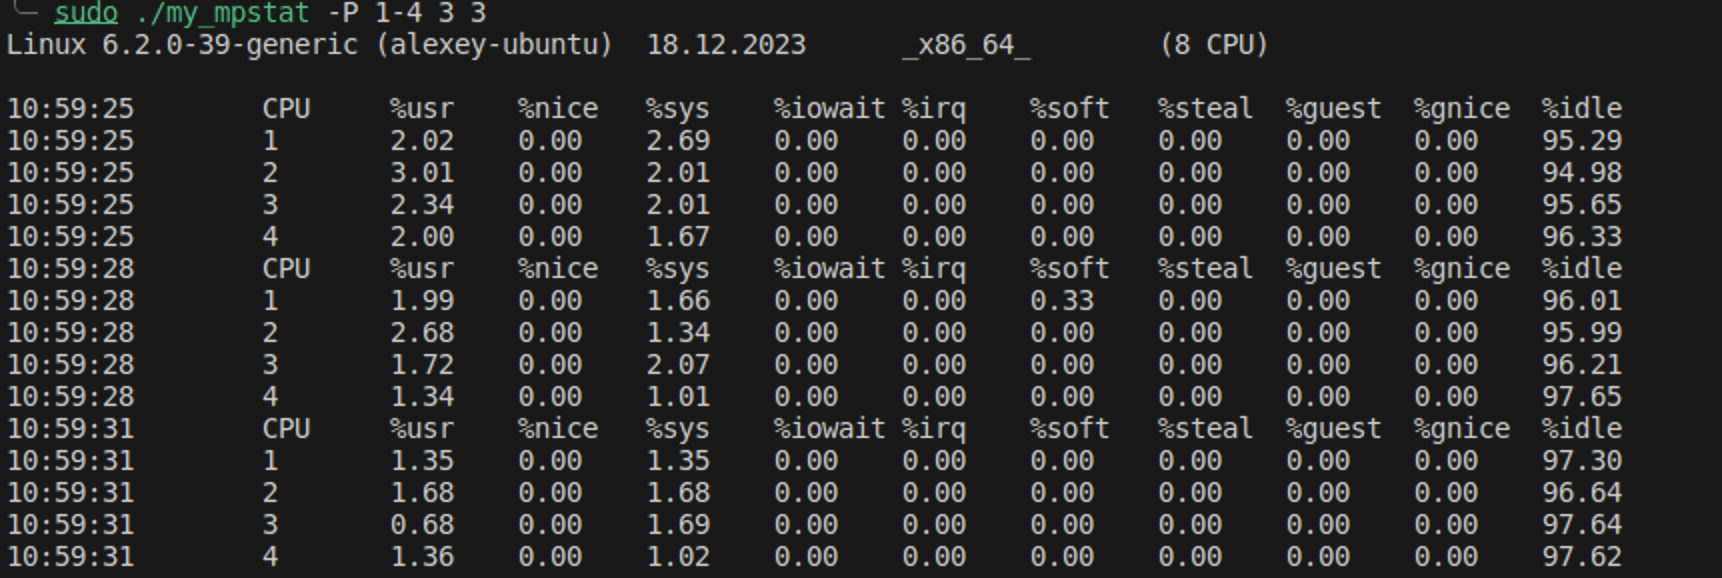
\includegraphics[width = \textwidth]{image/prog.png}


\section{Вывод:}
В ходе выполнения лабораторной работы я получил практические навыки по разработке комплекса программ на пользовательском уровне и уровне ядра. Этот комплекс программ собирает информацию на стороне ядра, передает ее на уровень пользователя и выводит в удобном для чтения виде. Для этого был разработан загружаемый модуль ядра и программа на уровне пользователя, которые взаимодействуют через интерфейс передачи \textbf{ioctl}. В результате выполнения лабораторной работы я получил практический опыт работы с ядром операционной системы.
\end{document}
